% !TeX root = ../main.tex
\section{Introduction}
\label{sec:introduction}
\subsection{Preparing for the Whole Opening}
A mobile robot can reach a handle and establish a firm grasp yet stop halfway
through opening the door. The handle follows an arc around a passive hinge;
as the arc progresses, the robot needs sufficient joint travel and stable
finger contact. Figure~\ref{fig:joint_limit} shows an example in which the door
reaches only $42.51^\circ$: bilateral contact persists, but the next inverse
kinematics (IK) target exceeds the available joint range. Preparation must
therefore account for the entire continuation.

Visibility creates a second dependency. An obstacle hidden from the initial
camera can change which side of the door is useful. Moving to inspect it
provides information, but also consumes travel and time. After choosing a
station, the robot acquires another view before selecting its grasp. These
decisions form a chain: inspection changes the information used for positioning,
and positioning changes the observations and motions available to grasping.
Skill chaining \citep{chen2023sequential} and active perception
\citep{bajcsy1988active} motivate treating these transitions as part of the task.

\ifshowfigures
% Recorded fixed-base diagnostic.
\begin{figure}[tbp]
  \centering
  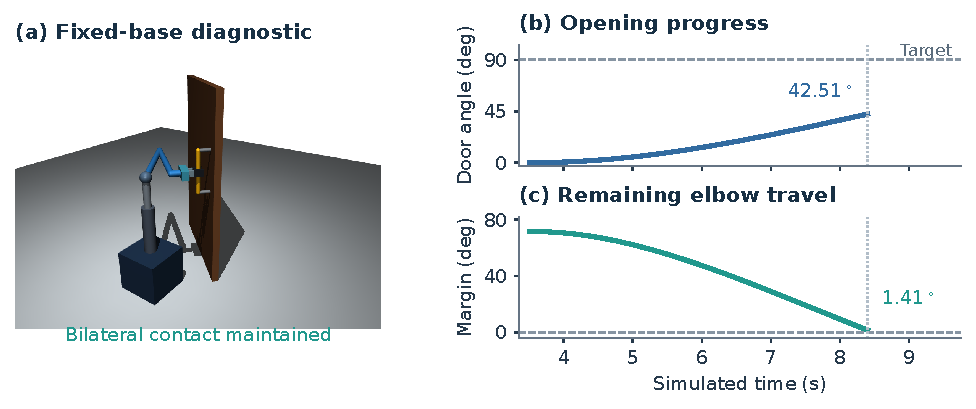
\includegraphics[width=\linewidth]{figures/failures/report_joint_limit.pdf}
  \caption{Fixed-base joint-limit diagnostic. (a) Recorded stopping configuration; (b) door opening; (c) remaining elbow travel. Bilateral contact persists at $42.51^\circ$ with $1.41^\circ$ of elbow margin. The next IK target exceeds the joint range and is rejected.}
  \label{fig:joint_limit}
\end{figure}

\fi

\subsection{Questions and Contributions}
We study how station selection should account for the executing grasp policy,
when inspection pays for itself, and which failures remain along the chain.
Our contributions are a continuous pipeline with reached observations,
downstream-conditioned supervision with staged LoRA, and matched test
comparisons of correctness and observation cost. The latest policy makes
$70/72$ correct decisions with 29 fewer inspections than always inspecting.
